\section[Introdução]{Introdução}

Em ambientes dinâmicos como feiras setoriais, visitantes e expositores enfrentam frequentemente dificuldades relacionadas à localização precisa dos fornecedores e ao registro eficiente de contatos, fatores críticos para o sucesso desses eventos. Atento a essa necessidade, o \textit{stakeholder} Igor Daudt idealizou o desenvolvimento de um totem interativo, projetado para superar esses desafios. O sistema proposto visa facilitar a interação dos visitantes com expositores por meio de um mapa tridimensional imersivo, tornando a experiência mais intuitiva e prática.

Com uma aplicação \textit{off-line} \textit{touch-screen}, o totem permitia que usuários buscassem facilmente produtos e fornecedores específicos em um ambiente visualmente atraente e interativo. O registro automatizado de visitantes por meio da leitura dos crachás otimizava significativamente a captura de contatos, e posteriormente relatórios detalhados foram entregues aos expositores, oferecendo \textit{insights} valiosos.

A execução do projeto ocorreu no primeiro semestre de 2025, entre os dias 28 de fevereiro e 27 de junho de 2025, compreendendo diversas etapas realizadas pelos estudantes do bacharelado em Engenharia de Software no âmbito da \ac{ages}, sob a orientação do professor Dr. Azriel Majdenbaum. A foto do time responsável pelo projeto pode ser vista na Figura~\ref{fig:totem-time}.

\begin{figure}[H]
    \centering
    \small
    \caption{Time do projeto Totem Interativo}
    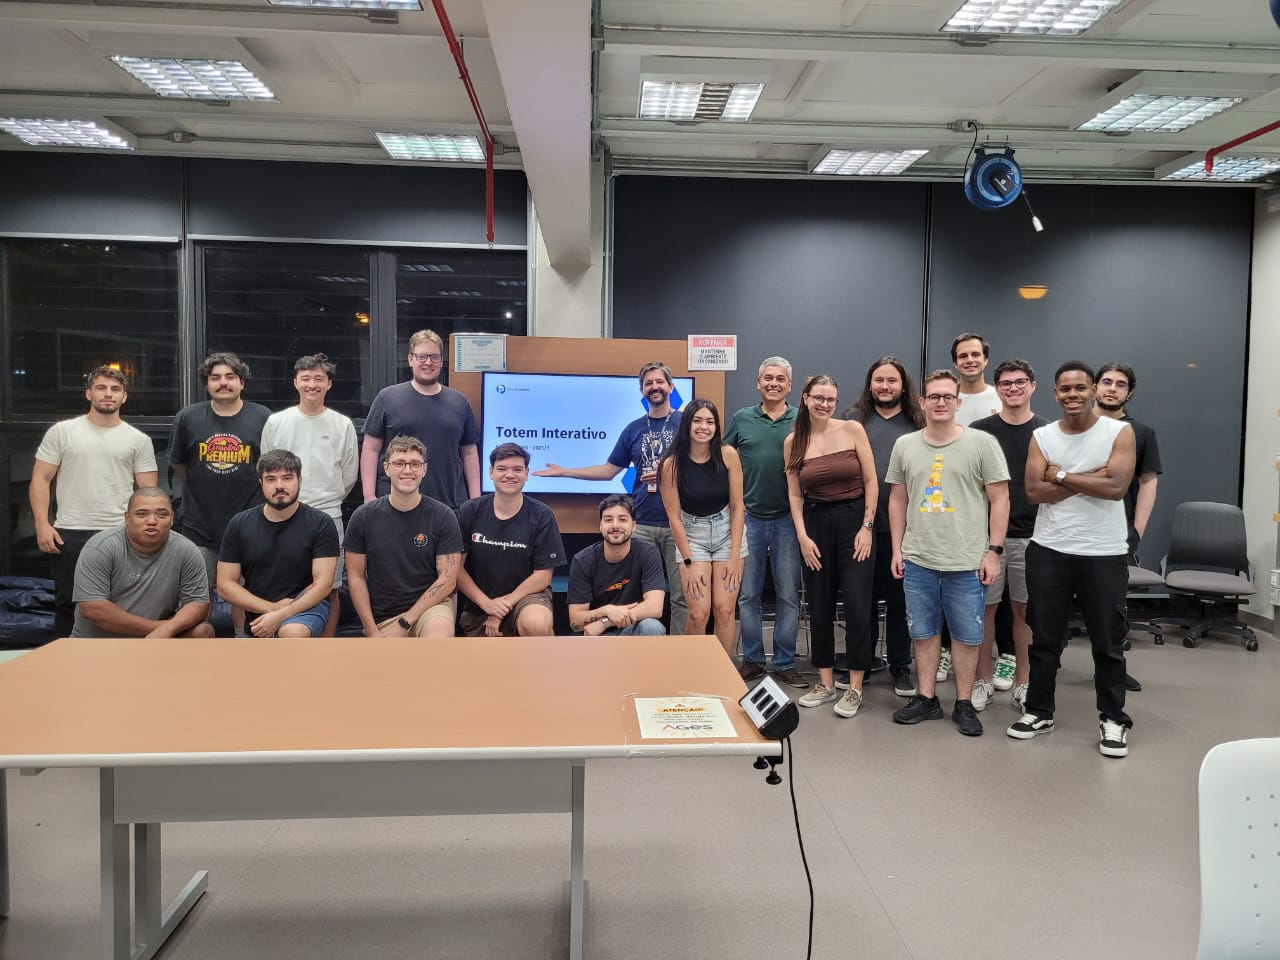
\includegraphics[width=0.9\linewidth]{conteudo/4 - ages III/images/fig6-time.jpg}

    Fonte: Wiki do projeto
    \label{fig:totem-time}
\end{figure}